\documentclass [a4paper, 12x `pt]{article}
\usepackage [utf8] {inputenc}
\usepackage [T2A] {fontenc}
\usepackage [russian] {babel}
\usepackage {amsmath, amsfonts, amssymb, amsthm, mathtools, textcomp, stmaryrd}
\usepackage{graphicx}
\usepackage{float}
\usepackage{wrapfig}

\title{Начало Математического безумия!}
\author{Александров Олег}

\begin{document}
\maketitle

Наше выражение: 
$$ \sin(x) ^{3}  + \cos(x) ^{3}  $$\\
Методом пристального взгляда заметим, что!
$$ \sin(x) ^{3}  + \cos(x) ^{3}  $$\\
"ДИРИРХЛЕЕЕЕ!!! ДИРИХЛЕЕЕ!!!" - Савватеев А.В.
$$ \frac{d}{dx}(x) = 1 $$\\
Наносим 10 Сталинских ударов по этому выражению!!!
$$ \frac{d}{dx}(\cos(x) ) = -1 \cdot 1 \cdot \sin(x)  $$\\
Вспоминаем метод Алекса Эдуардовича Султанова!!!
$$ \frac{d}{dx}(3) = 0 $$\\
Что это такое? А! Так это очевидно!!!
$$ \frac{d}{dx}(\cos(x) ^{3} ) = \cos(x) ^{3}  \cdot \left(0 \cdot \ln(\cos(x) )  +  \frac{3 \cdot -1 \cdot 1 \cdot \sin(x) }{\cos(x) } \right) $$\\
Получим вот такое выражение! Мы упустили часть доказательств равносильных переходов! Поэтому я хочу, чтобы ВЫ САМИ ИХ ДОКАЗАЛИ!
$$ \frac{d}{dx}(x) = 1 $$\\
Заметим, что ...
$$ \frac{d}{dx}(\sin(x) ) = 1 \cdot \cos(x)  $$\\
Сейчас наступит катарсис!!!
$$ \frac{d}{dx}(3) = 0 $$\\
Наносим 10 Сталинских ударов по этому выражению!!!
$$ \frac{d}{dx}(\sin(x) ^{3} ) = \sin(x) ^{3}  \cdot \left(0 \cdot \ln(\sin(x) )  +  \frac{3 \cdot 1 \cdot \cos(x) }{\sin(x) } \right) $$\\
Вас ещё не кокнуло? Продолжаем!
$$ \frac{d}{dx}(\sin(x) ^{3}  + \cos(x) ^{3} ) = \sin(x) ^{3}  \cdot \left(0 \cdot \ln(\sin(x) )  +  \frac{3 \cdot 1 \cdot \cos(x) }{\sin(x) } \right) + \cos(x) ^{3}  \cdot \left(0 \cdot \ln(\cos(x) )  +  \frac{3 \cdot -1 \cdot 1 \cdot \sin(x) }{\cos(x) } \right) $$\\
Производная выражения: 
$$ \sin(x) ^{3}  \cdot \left(0 \cdot \ln(\sin(x) )  +  \frac{3 \cdot 1 \cdot \cos(x) }{\sin(x) } \right) + \cos(x) ^{3}  \cdot \left(0 \cdot \ln(\cos(x) )  +  \frac{3 \cdot -1 \cdot 1 \cdot \sin(x) }{\cos(x) } \right) $$\\
Заметим, что ...
$$ \sin(x) ^{3}  \cdot  \frac{3 \cdot \cos(x) }{\sin(x) }  + \cos(x) ^{3}  \cdot  \frac{3 \cdot -1 \cdot \sin(x) }{\cos(x) }  $$\\
\begin{figure}
	\centering
	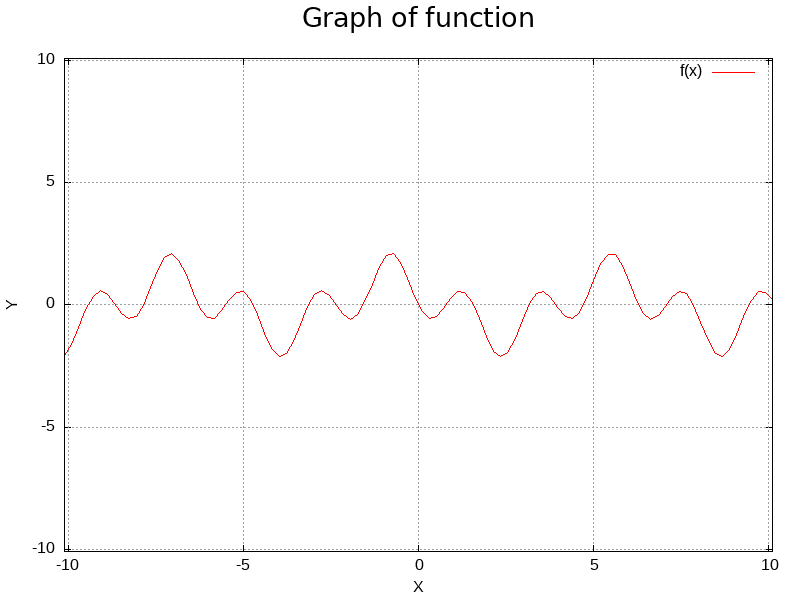
\includegraphics[width=0.5\linewidth]{Images/graphic.png}
	\caption{\label{fig:func}Graph of function.}
\end{figure}

\end{document}
